\subsection{Subjects}

Data were collected in four adult male rhesus macaques (Macaca mulatta)(“PO, CA, BU, and MO”) weighing 8–10 kg. 
All experimental procedures were approved by the Animal Care and Use Committee of the National Eye Institute and complied with the regulations of the National Institutes of Health. 
Plastic headposts were mounted with sterile surgical procedures, using procedures described in detail elsewhere \citep{lafer-sousa_parallel_2013}. 
The animals were acclimatized with positive reinforcement to sit in a custom-made chair positioned with the eyes 70cm in front of a computer monitor and to perform visual tasks as described below. 
At the beginning of each testing session, we positioned a mouthpiece to deliver fluid reward to the animal. 
An infra-red camera was directed at the eye to monitor eye position with the ISCAN system. 
The precision of the eye tracking was \textasciitilde0.3 degrees. 

\subsection{Behavioral task}

The animals were trained to perform a 4-Alternative Forced Choice (4-AFC), Delayed Match to Sample task, in which they were shown a colored cue and rewarded for selecting the match option that had the identical color (see Figure 1). 
The colors, described in more detail below, were drawn from a set of 64 colors that evenly sample hue angle of CIELUV color space \citep{stockman_colorimetry_2010}. 
Each trial was initiated when the animal fixated a small cross at the center of the screen; trials were aborted if the animal did not maintain fixation until the fixation cross disappeared toward the end of the trial. 
Fixation was defined as within a 1.5 degree wide area centered on the fixation cross, well within the precision of the eye tracker.
The trial sequence was as follows. 
Fifty ms after initiating the trial by fixating the central cross, a 3-degree-diameter “cue”  of a color randomly drawn from the set of 64 colors appeared for 750ms. 
The cue was positioned on the monitor at the same location for all trials during a given daily recording session.
From day to day, the position of the cue could vary, from 2.5-degrees to 6-degrees eccentricity (measured at the center of the cue) and be at any angle from fixation.
The cue was followed by a gray screen for a brief “memory” period of 600-900ms, after which four match options appeared along an arc at an eccentricity of 6-degrees. 

One match option was always a direct match to the cue, and the other three were randomly sampled without replacement from the remaining 63 stimuli. The match options had the same shape and size as the cue (3-degree-diameter discs); they were evenly spaced along the arc, with a gap of 2 degrees separating each option. In all animals except one (CA), the arc along which the match options were placed was in the visual hemifield opposite to the cue. The exact position of the arc within the hemifield varied from trial to trial, so the animals could not anticipate where the choice options would appear. Animal CA had a small scotoma spanning \textasciitilde3degrees of visual angle in a quarter of the visual field as the result of a \textasciitilde3mm diameter V1 lesion, so the cue and choices were placed in the same (intact) hemifield, taking care to avoid overlap of the position of the cue and the choices. 

After a random period from 500-1000 ms, the fixation cross disappeared, instructing the monkey to direct its eyes to one of the choices. This random period helped guard against the animals making impulsive responses because they could not anticipate when exactly the choice options would appear. Reward was given only if the animal selected with an eye movement the choice that was identical to the cue. 
If the monkey failed to make a choice within 5 seconds or broke fixation at any point before the termination of the fixation cross, the trial was aborted.

The experiment was controlled with custom software written in MATLAB and Psychtoolbox \citep{noauthor_nei-lsrkofiko_2022, kleiner_whats_2007}.

\paragraph{Stimuli}
Stimuli were 3-degree diameter discs presented on a Cambridge Research Systems Display++ screen. 
Colors were defined to be on an equiluminant plane in CIELUV color space, with the luminance matched to the adapting gray background (L* = 76.0693, 38.5cm/m2; adapting field chromaticity was xy\textsubscript{1931}: 0.2684, 0.2409). 
The stimulus set included 64 colors, evenly sampling CIELUV hue angle (5.625-degrees between adjacent stimuli), of equal CIELUV saturation (radius 37), the highest saturation possible for a set of stimuli of equal saturation and luminance given the gamut of the display.
Luminance contrast noise was randomly added to each pixel of the cue and the match options to mitigate chromatic aberration. 
The luminance added to each pixel was updated every frame and drawn uniformly from a continuous range of +/- 5 L* units (the resulting stimulus looks like a colored disc viewed behind a thin veil of television snow). 
CIELUV was used to define the stimuli because it has an associated chromaticity diagram, but the stimuli can readily be transformed into other spaces such as CIELAB and DKL. 

The color stimuli corresponding to the poles of the cone opponent cardinal axes, labeled in the polar mixture model plots, were computed as follows. 
CIELAB and CIELUV values were transformed to XYZ coordinates using the PsychToolbox functions “LabToXYZ” and “LuvToXYZ” respectively.
An XYZToLMS matrix was constructed using MATLAB's “mldivide” function with the Smith-Pokorny cone fundamentals and the CIE XYZ standard observer color matching functions as inputs.
The PsychToolbox function “ComputeDKL\_M” was then used to compute a conversion matrix for converting between LMS and cone opponent cardinal axes that define the DKL colorspace. 
The code which accomplishes the above is available \href{https://github.com/NEI-LSR/MacaqueColorCategories/blob/main/Analyses/DKL/computeDKL_XYZ.m}{here}.

\paragraph{Human Data}

Data from published reports using two related tasks completed in human subjects were kindly provided by Gi-Yeul Bae \citep{bae_why_2015} and Timothy Buschman \citep{panichello_error-correcting_2019}.
Both these data sets involved a paradigm in which participants matched the color of a cue to a ring of colors showing a continuous progression of colors around the color circle (a ``color wheel''). 
The results of the two prior studies are consistent with each other: when analyzed with a mixture model, both data sets show four color categories corresponding to blue, green, orange, and pink (SI Figure 1); moreover, the results on a version of the task that omits the memory delay period also recover these four color categories \citep{bae_why_2015}.
This prior work shows that the results on the color-matching task are reproducible and robust. 
It is therefore likely that the results of the present version of the task, which is distinguished from the prior work by providing as options discrete targets as opposed to a continuous colored wheel, would also be similar. 
But to test this likelihood, we recruited human participants via Amazon Mechanical Turk to perform the same task used in the macaque monkeys in the present work. 
To request a trial, participants used a mouse to adjust the location of a cursor to click on a fixation cross, after which a cue was shown to one side of the fixation cross, and the cursor disappeared. The cue was displayed for 750 ms. 
After the cue was extinguished, a fixation cross was shown but the cursor remained hidden to de-incentivize mouse movement (1500 ms). Four choices were then shown, and the cursor reappeared; participants made their selection by using the mouse to move the cursor to their choice and clicking the mouse. 
All other aspects of the experimental design were the same as the experiment deployed with the monkeys: 64 colors of equal saturation and luminance (we assumed the monitor that each on-line participant was using matched the sRGB standard), evenly sampling CIELUV. 
The pattern of results was consistent with the published studies using the continuous ring of colors, recovering four significant color categories corresponding to blue, green, orange, and pink (SI Figure 1; see Data Analysis: Mixture Modeling for a description of how these data were analyzed). %!!!!!!

\subsection{Data Analysis}

\paragraph{Psychometric functions}

Psychometric functions (see Figure 2a, SI Figure 2) were estimated with a Weibull cumulative density function: %!!!!

\begin{equation} \label{eq:Weibull}
    y=\zeta+(100-\zeta-\gamma) *\left(1-e^{-(\omega / \lambda)^k}\right) 
\end{equation}

Where animal performance (y) is a function of trial difficulty ($\omega$), computed for each trial as the angular difference between the color of the cue and the color of the foil with the closest color to the cue. 
The other parameters are the floor of the function ($\zeta$), the ceiling ($\gamma$), slope ($\lambda$), and inflection point ($k$). 
All completed trials were included in the analysis of the psychometric functions. 
The number of completed trials for each animal were: 76121 (PO); 54555 (CA); 24526 (BU); 54252 (MO). 

\paragraph{Mixture Modeling}\label{para:MixtureModeling}

Following experiments in human subjects, we analyzed the distribution of color matches made to each color using a mixture model \citep{zhang_discrete_2008,bae_why_2015}; this model assumes that the shape of the distribution is normal and provides an estimate of the width of the distribution, the offset (or bias) of its peak relative to the target color, and the guess rate.
Prior work has done this analysis with a von Mises distribution \citep{zhang_discrete_2008,bae_why_2015}.
We found it simpler to implement it with a Gaussian function, $f(\theta)$:

% demo annotated-equation code from here: https://mirrors.concertpass.com/tex-archive/macros/latex/contrib/annotate-equations/annotate-equations.pdf

%\newpage %Sometimes the annotations don't show up, the hacky solution is to force them onto a new page

\begin{equation} \label{eq:GaussianEquation}
    f(\theta) = {\alpha} \cdot e^{-\frac{(\theta-{\mu})^2}{2{\sigma}^2}} + {\zeta}        
\end{equation}

% \vspace{2em} 
% \begin{equation} \label{eq:GaussianEquation}
%     f(\theta) = 
%     \eqnmarkbox[purple]{alpha}{\alpha}
%     \cdot
%     e^{
%     -\frac{(x-
%     \eqnmarkbox[violet]{mu}{\mu}
%     )^2}{2 
%     \eqnmarkbox[blue]{sigma}{\sigma}^2}}
%     +
%     \eqnmarkbox[gray]{zeta}{\zeta}        
% \end{equation}

%\annotate[yshift=1em]{above,left}{alpha}{height of the curve's peak}
%\annotate[yshift=1em]{above}{mu}{position of the center of the peak}
%\annotate[yshift=-0.75em]{below,left}{sigma}{standard deviation}
%\annotate[yshift=-1em]{below}{zeta}{floor}
%\vspace{2em} 

where $\alpha$ is the height of the curve's peak, $\theta$ is the hue angle, $\sigma$ is the standard deviation (width), $\mu$ is the center of the peak (so the offset is $\theta$-$\mu$), and $\zeta$ is the floor (guess rate). 
To do the analysis, we used the MATLAB fit function, which was provided with the number of times each choice color was an option for the given cue across all completed trials and produced the best-fitting function along with the 95\% CI values for those parameters (SI Figure 3; note that the tails of the distributions in SI Figure 3 reach an asymptotic floor, justifying the use of the simpler Gaussian fitting procedure). 
The offset values for each cue were smoothed with a moving average spanning three colors (16.875 degrees) (Figure 2b and 2c, Figure 5a, and SI Figure 4). Negative-slope zero-crossings in which the 95\% CI exceeded the zero crossing were considered category centers (see Figure 1).

The width of distribution of matches varied among the colors; this was also observed by \citet{bae_why_2015} (see their Figure 7). 
This variation implies that the assumption of uniformity of the colorspace is not valid. 
Moreover, such a non-uniformity could yield an offset in the mixture model (see Figure 3), so any offsets recovered by the mixture model need not require a cognitive origin.  
The alternative hypotheses for the origin of offsets recovered by the mixture model (a cognitive origin versus a stimulus-space non-uniformity), prompted us to analyze the data with a more sensitive model, the Target Confusability Competition model \citep{schurgin_psychophysical_2020}.
We recognize that in principle, the mixture model could distinguish these alternative hypotheses, but we encountered some limitations using the mixture model that were readily overcome by the TCC model. 

\paragraph{Modified Target Confusability Competition Model (TCC-v)}\label{para:TCC}

The key elements of the TCC model are a similarity function, which determines the similarity between stimulus $s_i$ and stimulus $s_j$ through a non-linear mapping of distance in colorspace to perceptual similarity, and a value of $d'$, which can be thought of as describing the amount of noise acting in the system. 
These two elements can be used to predict the probability that a choice of colour $s_j$ will be picked from the set of $\left[s_{j1}...s_{jn}\right]$, on a trial where the cue is $s_i$. 

The probability of a particular choice being selected on a particular trial ($p_t(\text{selecting choice}_n)$) is dependent on the cue, the set of choices, the similarity function ($f(\theta)$), the value of $d'$, and the perceptual distances between stimuli ($D$).

\begin{equation} \label{eq:pt}
    p_t\left(\text{selecting choice}_n \mid \text{cue},\text{choices}_{i:j}, f(\theta), \delta, D\right)
\end{equation}

where $f(\theta)$ is the Gaussian equation (\autoref{eq:GaussianEquation}), $\delta$ is the value of $d'$, and $D$ is the perceptual distances between stimuli.

The TCC model has been deployed with the assumption that the colorspace is perceptually uniform \citet{schurgin_psychophysical_2020}; this assumption is implemented as a single similarity function fit for all stimuli. 
But, as \citet{schurgin_psychophysical_2020} demonstrate the similarity function need not be fixed (see their Figures 1d and Extended Data Figure 5). 
Our implementation of the model, which we call TCC-v, permits the similarity function to vary for each cue (the "v" is for vary). 

We created four versions of the TCC-v model: the "null model" (with only parameters for the Gaussian width of the similarity function and $d'$, and thus no allowance for bias), the "cognitive bias" model (with 64 parameters corresponding to offset values shifting the peak of the similarity function for each stimulus to higher or lower hue angles, in addition to $d'$ and gaussian width), and the "stimulus-space non-uniformity model" (with 64 parameters corresponding to the relative distance between each pair of neighboring stimuli, in addition to $d'$ and gaussian width). 
Finally, the "free-similarity" model, does not pre-suppose any specific similarity function; every cell in the similarity matrix is an independent parameter. 
This flexibility allows for patterns of similarity that are not captured by our hypotheses. 

In fitting the model parameters, our goal is to minimize the negative log likelihood (NLL) of the observed data. 
The NLL is computed as the sum of the negated log of the probabilities of the choices that were selected being selected. 

\begin{equation}
    \text{NLL} = \operatorname{sum}\left(-\left(\log \left(p_t\left(\text {selecting choice}_x\right)\right)\right)\right)
\end{equation}

where $\text{choice}_x$ was the choice that was selected on each trial.

The parameter estimates for the free parameters used by the model are iteratively updated until the model reaches a stable minimum NLL. 

The "null model" is defined by $f(\theta)$ (where $\alpha$ = 1, $\zeta$ = 0, $\mu$ = 0) and $d'$, and assumes $D$ to be uniform. 
The "cognitive bias" model is defined by $f(\theta)$ (with 64 parameters for $\mu$, 1 parameter for $\sigma$, $alpha$ = 1, $\zeta$ = 0) and $d'$, and also assumes $D$ to be uniform. 
The "stimulus-space non-uniformity" model is defined by $f(\theta)$ (where $\alpha$ = 1, $\zeta$ = 0, $\mu$ = 0) but specifies for each pair of neighboring stimuli a unique value for $D$ (64 parameters). 
Note that the cognitive bias model and the stimulus-space non-uniformity have the same total number of parameters (66). 
The "free similarity model" is not defined by $f(\theta)$; it is defined by $d'$ and the similarity matrix. 
The similarity matrix is defined by 4096 ($64^2$) parameters, one for each combination of cue and possible choice (note that the free similarity matrix is not required to be symmetric).

$p_t(\text{selecting choice}_n)$ is the probability that a sample drawn from an independent normal distribution $(X_i \sim N)$ is the highest of such samples drawn for all the choices ($i:j$) on a particular trial. 
The mean ($m$) of each distribution is defined by the similarity value for that cue/choice combination, multiplied by $d'$, and has a variance of 1.

\begin{equation}
    p\left(\text{selecting choice}_n\right) = 
    p\left(X_i \sim \mathcal{N}\left(m_n \cdot \delta, 1\right)
    >\max 
    \left(X_{i+1: n} \sim \mathcal{N}\left(m_n \cdot \delta, 1\right)\right)\right)
\end{equation}

where $m_{i:j} = f\left(|\text{cue}_{i} - \text{choices}_{i:j}|\right)$, and $\delta$ is the value of $d'$.

We used an AFC paradigm as opposed to a continuous response space, so we can take advantage of an alternative computational method for estimating $p_t(\text{selecting choice}_n)$, using correction factors provided by \citet{mcgraw_common_1992} (their Table 3). 
This decreases the amount of time taken to fit the TCC-v models. 
The method for computing $p_t(\text{selecting choice}_n)$ in the original TCC model of Schurgin et al. is provided here: \verb|modelPDF| in \verb|TCC_Code_InManuscriptOrder |\verb|\Model| \verb|\TCCUncorrelated.m| from \url{https://osf.io/j2h65/}. 
The method we used is provided here: \url{https://github.com/NEI-LSR/TCC_AFC}.

When fitting the free similarity matrix model, we fix $d'$ to provide a constraint on the floor and ceiling of values in the similarity matrix.
$d'$ is strongly correlated with the range of the values in the similarity matrix; the range of similarity values in the similarity matrix has a maximum span of 0 to 1. 
Equivalent NLL values can be obtained either by restricting the range (e.g. 0.49 to 0.51) and a high value of $d'$ (e.g. 20), or by having a larger range (e.g. the full 0 to 1) and a low value of $d'$ (e.g. 0.1). 
If $d'$ is not fixed, the model is as likely to assume a restricted range as it is a larger range (though still bounded between 0 and 1) but will take a long time to converge. 
Fixing $d'$ impacts the specific values (akin to increasing or decreasing the contrast of the similarity matrix image) but it does not impact the interpretation of the similarity matrix. 
We chose a $d'$ value of 1 which is a reasonable estimate for our task \citep{schurgin_psychophysical_2020}.

In the original TCC model, the similarity function uses two parameters that define a Gaussian function representing perceptual noise and an exponential function; these two functions are convolved (see Figure 1f of \citep{schurgin_psychophysical_2020}). 
We simplify the similarity function such that it is defined by a Gaussian alone. 
The cost of this is that it does not allow for a distinction between the impact of perceptual noise (where the curve flattens off approaching perceptual distances of 0) and similarity (the general shape of the function). 
In practice, we found that these parameters were highly correlated, and that reduction to a single parameter substantially reduced the computational cost of model fitting, and produced parameter estimates that were more resistant to variation in model-fitting starting values. 
This simplification also made it easier to modify the model; for example, to allow for the peak of the function to not be at 0 (this affords the TCC-v model the same ability as the mixture model to capture offsets).

\paragraph{Choice Probability Matrices vs. Similarity Matrices}

\begin{figure}
    \begin{fullwidth}
    \centering
      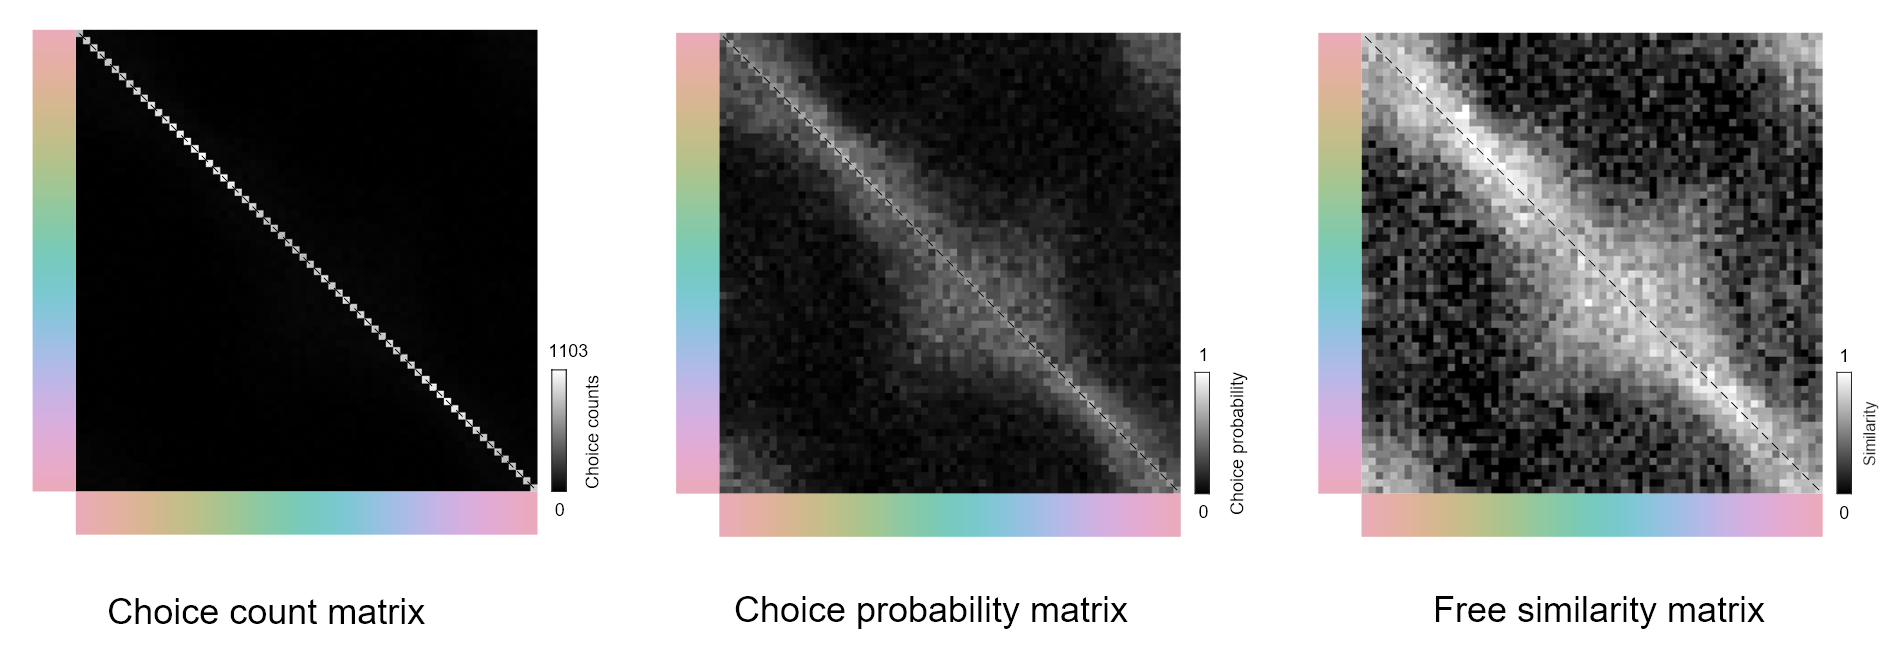
\includegraphics[width=\textwidth,]{../Figures/flat/F7_choiceProbVsSim.png}
           \caption{\textbf{Comparison of Choice Count Matrices, Choice Probability Matrices, and Similarity Matrices}.
           Choice count matrices describe the number of times a specific choice is made. 
           Choice probability matrices normalise for the number of times a particular choice was available as a choice option. 
           Similarity matrices are created through model fitting and represent the perceptual similarity between stimuli, and are beneficial since they are not influenced by mixed viability of distractors (see text for further details).}
		\label{fig:MACBEHcolorspace}
    \end{fullwidth}
\end{figure}

A choice probability matrix is a graphical representation of the probability that choice y will be chosen given cue x.
To construct such a matrix, one counts the choices which were made in response to each cue, producing what we can refer to as a choice count matrix, and then divides each cell by the number of times that each cue/choice combination was presented. 
This normalizes for the possibility that some cue/choice combinations were presented more than other combinations. 
This process disregards any information about what the unchosen distractors were on a given trial.

In paradigms which use a continuous response space the set of choices is the same on each trial – the full set of possible choices. 
This is not the case for our reduced AFC paradigm, and this introduces a potential issue which needs consideration.

Imagine a trial with three distractors which are all close to one another (let's say that they are 5, 6, and 7 colorimetric units away from the cue).
On another trial, imagine that one distractor is a much more viable choice option than the other two (let's say the choices are 5, 25 and 26 units away from the cue).
The odds of picking the distractor that is 5 units away is different on these two trials - it is more likely on the second trial, because the other distractors are less viable options. 
This becomes a potential issue because to counterbalance trials such that each cue is shown with the full set of possible distractors would require roughly 2.5 million trials (nchoosek(63,3) * 64).
Without counterbalancing, it is not possible to disentangle differences in choice probability which arise due to perceptual similarity (which is what we are aiming to measure) vs differences in distractor viability.

We avoid having to collect a complete set of 2.5 million trials by employing the concept of a similarity matrix.
A similarity matrix is the core component of a TCC-v model, and maps the similarity between cues and choices. 
Using it, the similarity between the cue and each of the choices on a particular trial (and also the similarity between each of the choices themselves) can be used to compute the probability of each choice being selected.
While we can compute the choice probability matrix rather simply, as described above, the creation of a similarity matrix requires a model-fitting approach – a similarity matrix is randomly initialized with values, and the likelihood of the data given that matrix is computed, then the matrix is randomly perturbed and the likelihood of the data is recomputed, and then perturbed again in whatever directions seem to increase the likelihood of the data, setting forth an iterative process whereby the similarity matrix is perturbed until a maximum in likelihood is reached, and our best estimate of the underlying similarity matrix is thus settled upon.
This is a computationally intensive process, and for datasets with many choices (such as those with a continuous response space), we have been unable to fit similarity matrices. 
Thankfully, there is a trade-off: data collected with continuous response spaces see less benefit of a similarity matrix over a probability matrix. 
For such datasets, as the number of trials increases the probability matrix increasingly approximates the similarity matrix.
It is expected that choice probability matrices and similarity matrices will be highly correlated and show the same structure.

A related issue, also addressed by employing the concept a similarity matrix, is the artifact caused by the inclusion of a direct match on every trial in our paradigm. 
This can be thought of as an unequal counterbalancing which no number of repeated trials would be able to balance out, but it is necessary for our training of the monkeys (since there needs to be a clear rubric for what choices are “correct” and thus rewarded).
Note how the choice count matrices and choice probability matrices for our data appear to show an elevated diagonal. 
The reason this exists in the choice count matrix is clear – those option are simply presented more frequently, but the reason this survives the normalization (by the number of times that each cue/choice combination was presented) is less obvious: any non-match choice which is close to the direct match will always have a viable competitor (the match), whereas the match choice won't always have a viable competitor (since it is possible that the distractors are all distant on a particular trial).
This leads to an increased probability of selecting the matching choice relative to an incorrect choice. This issue only affects choice probability matrices; it does not affect similarity matrices.

\paragraph{Quantitative Model Comparison}
To compare the relative performance of models, we computed Bayesian Information Criterion (BIC) values for each model from the NLL. 
The BIC values provide a unit by which we can assess whether the differences between NLL are meaningful, penalizing for number of parameters and number of trials. 
BIC also allows us to compare models with differing numbers of parameters (though note that the "cognitive bias" and "stimulus-space non-uniformity" models have the same number of parameters).

\begin{equation}
    \text{BIC} = k\ln(n)-2\ln(\hat{L})
\end{equation}

Where $\hat{L}$ is the maximised likelihood of the model, $n$ is the number of trials, and $k$ is the number of parameters.

To compare the relative performance of the cognitive bias and stimulus-space non-uniformity models we performed 100 bootstrap iterations of the analysis. 
Each bootstrap drew 24526 trials from the total number of completed trials for each animal (24526 was the minimum number of trials of completed trials among the 4 animals). 
Both models were then fit to each bootstrap iteration, and the BIC values were computed (see Figure 4d).

\paragraph{Reverse-engineering a uniform color space from the macaque color-matching data}

The present results imply that CIELUV is perceptually non-uniform; that is, that it samples with variable density the true underlying perceptual colorspace. 
The parameters of the stimulus-space non-uniformity model describe the relative positions of the stimuli, as determined empirically. 
After converting from inter-neighbor relative distances to polar angles, these can be thought of as the hue angles for the stimuli that we used, represented now in a behaviorally derived color space which we refer to as the Macaque Uniform Color Space (MUCS) (Figure 6b). 
The inverse transformation is also possible; we can define a set of hue angles that are uniformly distributed in MUCS and convert them into CIELUV. 
For example, if we define hue angle $i$ in MUCS, we can reparameterize that hue angle such that it is defined by its angle relative to the two experimental stimuli on either side of it (hue angle $i$ is at y\% of the angular distance on the path between experimental stimuli $a$ and $b$). 
We can then plot MUCS hue angle $i$ in CIELUV by plotting it at the location which is y\% along the path between experimental stimuli $a$ and $b$ in CIELUV. 
Such a set of hue angles is shown in Figure 6c. 

The MATLAB script MUCS.m will generate a user-defined number of colors sampled evenly from the behaviorally generated color space.
